\documentclass{article}

% Packages
\usepackage{amsmath}
\usepackage{pdfpages}
\usepackage{tikz}

\usepackage{markdown}

\usepackage[newfloat]{minted}     % Syntax highlighted code
\usepackage{xcolor}

\newenvironment{code}{\captionsetup{type=listing}}{}
\SetupFloatingEnvironment{listing}{name=Code}

\usepackage[hidelinks]{hyperref}

\usepackage{caption}
\usepackage{subcaption}

\usepackage{float}
\usepackage{graphicx}
\graphicspath{ {./images/}}

\usepackage{setspace}
\setstretch{1.5}

% Configuring biblatex
\usepackage[style=ieee]{biblatex}
\addbibresource{project_formulation/bib.bib}

% Configuring Fancy hdr
\usepackage{fancyhdr}
\pagestyle{fancy}

\fancyhead[R]{Bachelor Thesis}
\fancyhead[L]{Philip Oliver Mejer Jørgensen}

% Configuring title page
\title{\textbf{Detection of Vinyl Chloride in Environmental Water Samples}~\\[5mm]
\large{By: Philip Oliver Mejer Jørgensen}~\\[5mm]

\includegraphics[width=0.4\textwidth]{sdulogo.png}}
\author{
Supervisors:~\\[3mm]
Main supervisor: Associate Professor Roana de Oliveira Hansen~\\[15mm]
University of Southern Denmark (SDU)\\
Faculty of Engineering - Mechatronics\\
Sønderborg, Denmark
}
\date{January 2024}

% Main document
\begin{document}
\maketitle
~\\[2mm]
\begin{center}
\large{
Thesis submitted\\
as a part of the\\
Bachelor of Engineering in Mechatronics
}
\end{center}
\thispagestyle{empty}
\newpage

\addcontentsline{toc}{section}{Abstract}
\begin{abstract}
Abstract. write toward the end
\end{abstract}

\listoffigures

\addcontentsline{toc}{section}{Abbreviations}
\section*{Abbreviations}
\begin{tabular}{ll}
VOC     & Volatile Organic Compound \\
VC      & Vinyl Chloride \\
PVC     & Polyvinyl Chloride \\
GC      & Gas Chromatography \\
GSC     & Gas-solid Chromatography \\
GLC     & Gas-liquid Chromatography \\
EHP     & Environmental Health Perspectives \\
\end{tabular}
\newpage

\tableofcontents

\newpage

% The different sections to include:

\addcontentsline{toc}{section}{Project Formulation}
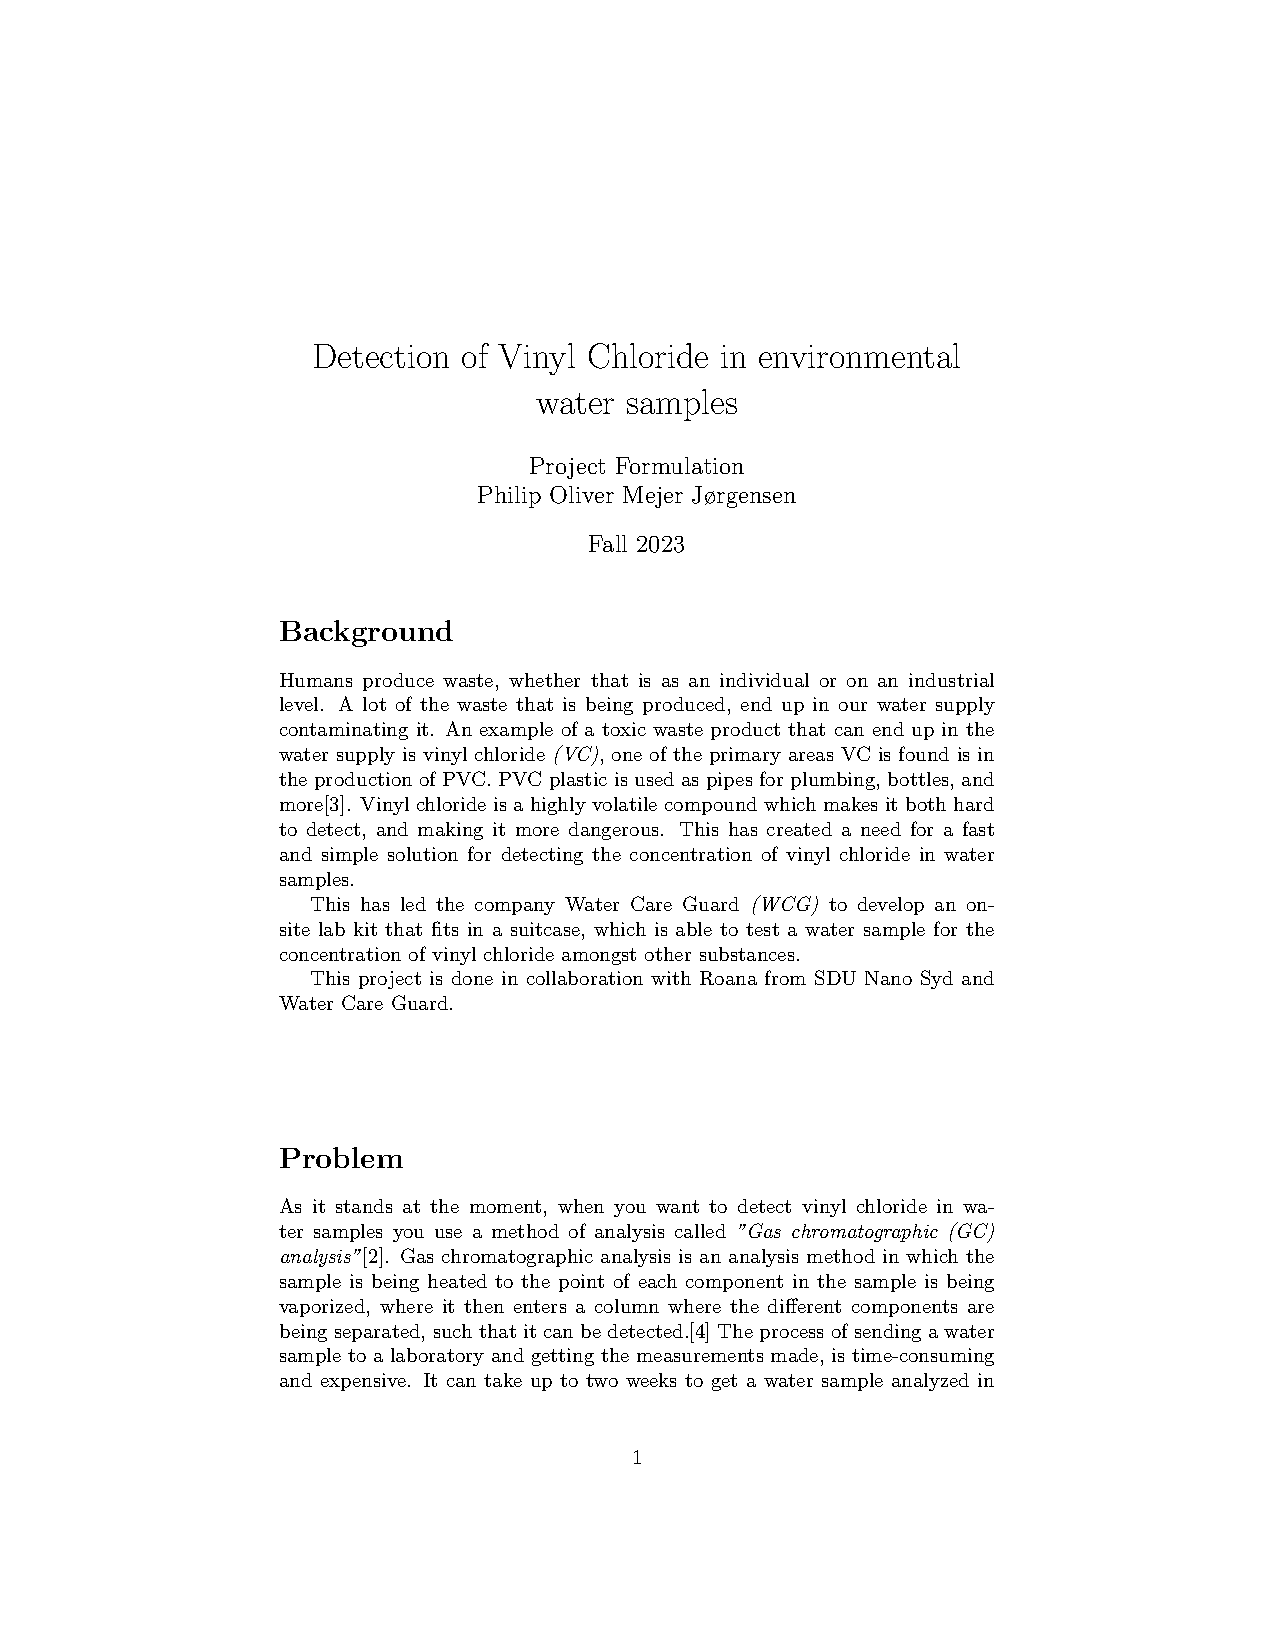
\includepdf[pages=-]{project_formulation/project_formulation.pdf}

\section{Introduction}
\subsection{Background}
Humans have been producing waste for a long time, but as the materials that we use change so has our waste.
In the early 20th century with the invention of fully synthetic plastic by the Belgian chemist Leo Baekeland in 1907\cite{plastic_history}, started a new type of anthropogenic pollution.
One type of plastic known as Polyvinyl Chloride (PVC), which was first synthesized in 1872 by Dr. Eugen Baumann\cite{pvc_origin}, it was first plastasized by Dr. Waldo L. Semon in 1926\cite{history_pvc}.
The introduction of plastics and especially PVC plastics, has introduced a new biproduct which is a highly toxic volatile organic compound (VOC), called Vinyl Chloride (VC).
Vinyl chloride is a biproduct in the production of PVC plastics, from it being used as the main component in the production of PVC plastics.
PVC plastics are used in a lot of different areas like construction piping, packaging, wires, toys, etc. in figure \ref{fig:pvc_applications} some examples of PVC applications are shown.

% Applications for PVC plastic figure
\begin{figure}[H]
    \centering
    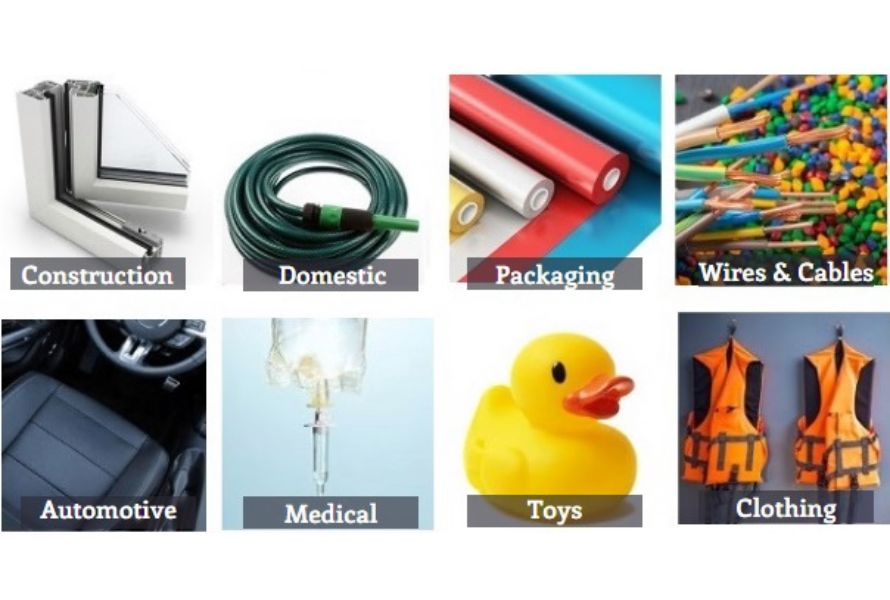
\includegraphics[width=0.7\textwidth]{pvc_applications.jpg}
    \caption{Applications for PVC plastic. \cite{pvc_applications_euroeplas}}
    \label{fig:pvc_applications}
\end{figure}

People can be exposed to vinyl chloride in different ways, through inhalating contaminated air, contaminated water etc.
If vinyl chloride contaminate a water supply to a household, it can contaminate the air in the household leading to the inhabitants being exposed to vinyl chloride. \cite{vc_cancer}
One of the main dangers with exposure to vinyl chloride is the increased risk of cancer, and in particular liver cancer.\cite{vc_cancer}
In addition according to \textit{"kemibrug.dk"}\footnote{A database for information regarding chemicals}, vinyl chloride can also affect the central nervous system with symptoms like headache, dizziness, nausea and a possibility of loss of conscioiusness, as well as the inhalation the chemical is also easily absorbed through the skin which can lead to similar effects as of those from inhilation.\cite{vc_kemibrug}\\


At the moment the primary way to analyze whether there is vinyl chloride present in a water sample is through gas chromatography.
According to an article from F.J Santos and M.T Galceran some of the advantages of gas chromatography are that is has a very high selectivity and resolution, making it easier to detect even small quantities of vinyl chloride in the sample, in addition GC has a good accuracy and precision.\cite{SANTOS2002672}\\


Gas chromatography is a physical process where a mixture of different substances are separated into their different parts.\cite{waters_1978_gc}
There are two primary types of gas chromatography, gas-solid chromatography (GSC) and gas-liquid chromatography (GLC), in gas-solid chromatography it is about the absorbtion of the sample on the solid and with gas-liquid chromatography it is about the solubility of the sample to the liquid. \cite{ambrose_1963_gc}
In the case of detecting the vinyl chloride it is GLC that is being used, since the sample to be tested for the concentration of vinyl chloride is usually water.
According to the "Environmental Health Perspectives (EHP)" some of the areas that there have been shown high levels of VC are "soil, groundwater, aquifiers, and wells near landfill and industrial waste disposal sites"\cite{vc_kielhorn_2000}.
Gas chromatography works by having a sample that is to be analyzed, that is injected into a moving gas stream.
It is then being carried down a column by a liquid with a low volatility, the sample is then separated into its different parts because the absorptivities and solubilities of the different parts differ making them arrive at different rates which makes it possible for the detector at the end to get a reading.\cite{ambrose_1963_gc}
The process is illustrated in figure \ref{fig:glc_illustration}.

\begin{figure}[H]
    \centering
    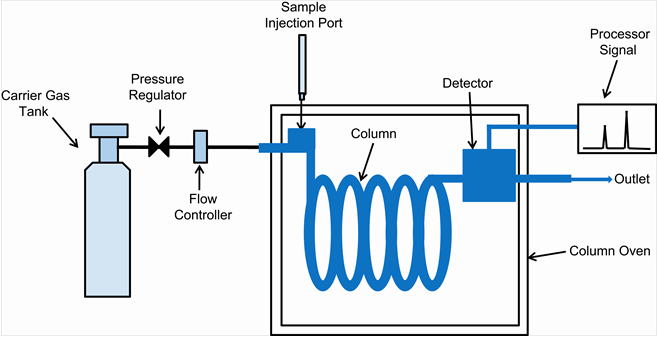
\includegraphics[width=0.9\textwidth]{glc_illustration.png}
    \caption{Schematic illustration of a gas chromatography system. \cite{glc_illustration}}
    \label{fig:glc_illustration}
\end{figure}

A gas chromatograph is an expensive piece of laboratory equipment\cite{gc_cost_axion}, in addition it can take up to two weeks to get a sample analyzed in a laboratory\cite{water_analysis_cwt}.
This is why there is a need to be able to get a faster on-site detection of vinyl chloride concentration in water samples.
This is what the company Water Care Guard\footnote{\url{https://www.watercareguard.com/}} is working towards, with their suitcase laboratory.
Instead of using GC for detecting the vinyl chloride, it is using an enzymatic reaction between the vinyl chloride and an enzyme (Cytochromes P450), this enzymatic reaction changes the refractive index of the solution over time where the shift in the refractive index from the starting point is related to the concentration of the vinyl chloride in the solution.\cite{roana_vc_ri}\cite{Ghanayem2007-nb}.

\newpage
\section{Theory}
This section will be explaining the relevant concepts, for the method that is used for detecting vinyl chloride in the Water Care Guard suitcase.

\subsection{What is \textit{Refractive index}?}
The definition of refractive index from The Britannica Encyclopaedia is:
\begin{center}
"measure of the bending of a ray of light when passing\\from one medium into another"\cite{ri_britannica}
\end{center}

The refractive index is defined as the the sine of the angle of incidence to the sine of the angle of refraction.\cite{ri_britannica}
Equation \ref{eq:ri} shows how the refractive index is calculated as either the ratio of the sine of the angles or as the ratio of the speed of light in a vacuum ($c$) over the speed of light in the medium ($v$).\cite{ri_mettler_toledo}
The angles, $i$ and $r$ are shown in figure \ref{fig:ri}.
\begin{equation}\label{eq:ri}
    n = \frac{\sin{i}}{\sin{r}} = \frac{c}{v}
\end{equation}

\begin{figure}[H]
    \centering
    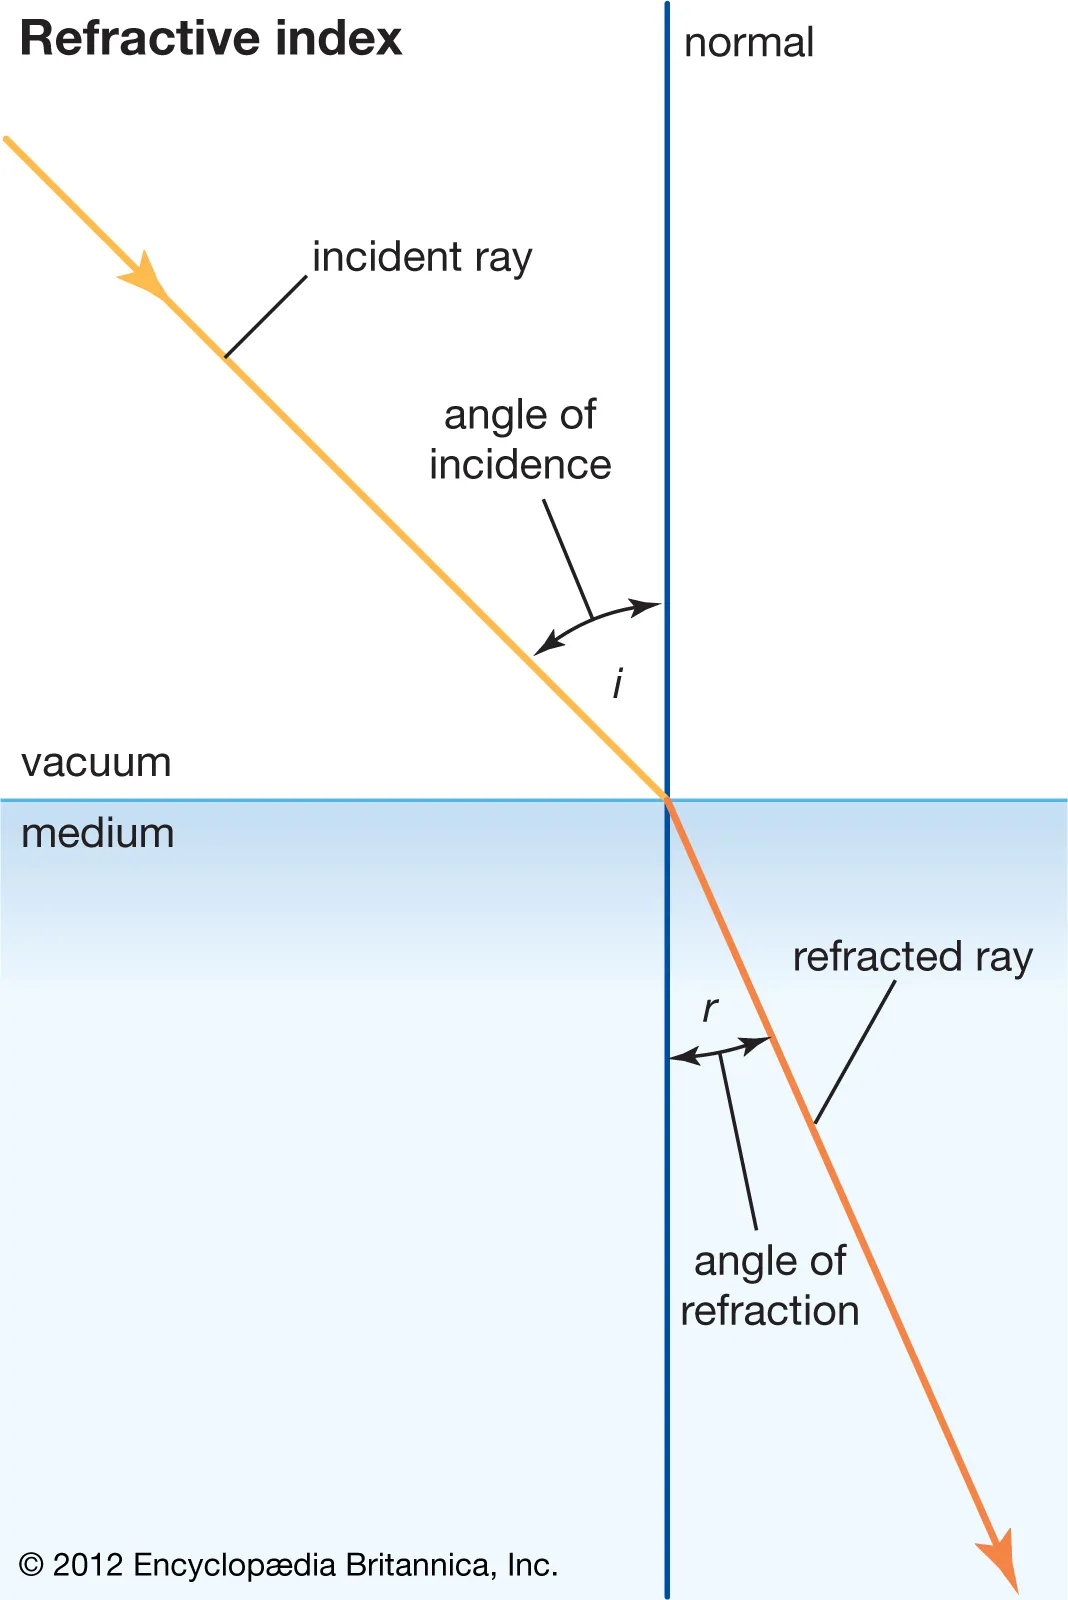
\includegraphics[width=0.5\linewidth]{refractive_index.png}
    \caption{An illustration of refractive index\cite{ri_britannica}}
    \label{fig:ri}
\end{figure}

When the vinyl chloride reacts with the enzyme Cytochrome P450, the refractive index of the solution changes with time as the components are reacting\cite{roana_vc_ri}.
Thus the refractive index can be used to determine the concentration of the vinyl chloride in the solution, as a more affordable alternative to using gas chromatography.

\subsection{The photonic cystals, a tool for measuring the refractive index}

\newpage
\section{Building a database}
\subsection{Measuring vinyl chloride in a sample}
\subsubsection{General methodology}

The methodology is derived from the methodology shown in the appendix \ref{appendix:protocol_vc}, with changes depending on the specific equipment and concentration values.\\

During the measurement gathering process, there was a procedure that was followed for all the measurements, it was adapted slightly depending on what instrument the measurement was done on.
Firstly the instrument was turned, and proceeding with the steps only when the instrument had heated up.
With the Water Care Guard suitcase or with the Ocean Optics UV-650 UV-VIS\texttrademark\, the heat up wait was a fixed 15 minute wait, because those instruments did not have a heating status indicator telling when it was finished heating up.
On the other hand with the Shimadzu UV-1900\texttrademark\, there is a light on the front indicating the status, if it is yellow it is still heating and green when it is ready, this is indicated in figure \ref{fig:shimadzu_status}.

\begin{figure}[H]
    \centering
    \begin{subfigure}[b]{0.48\textwidth}
        \centering
        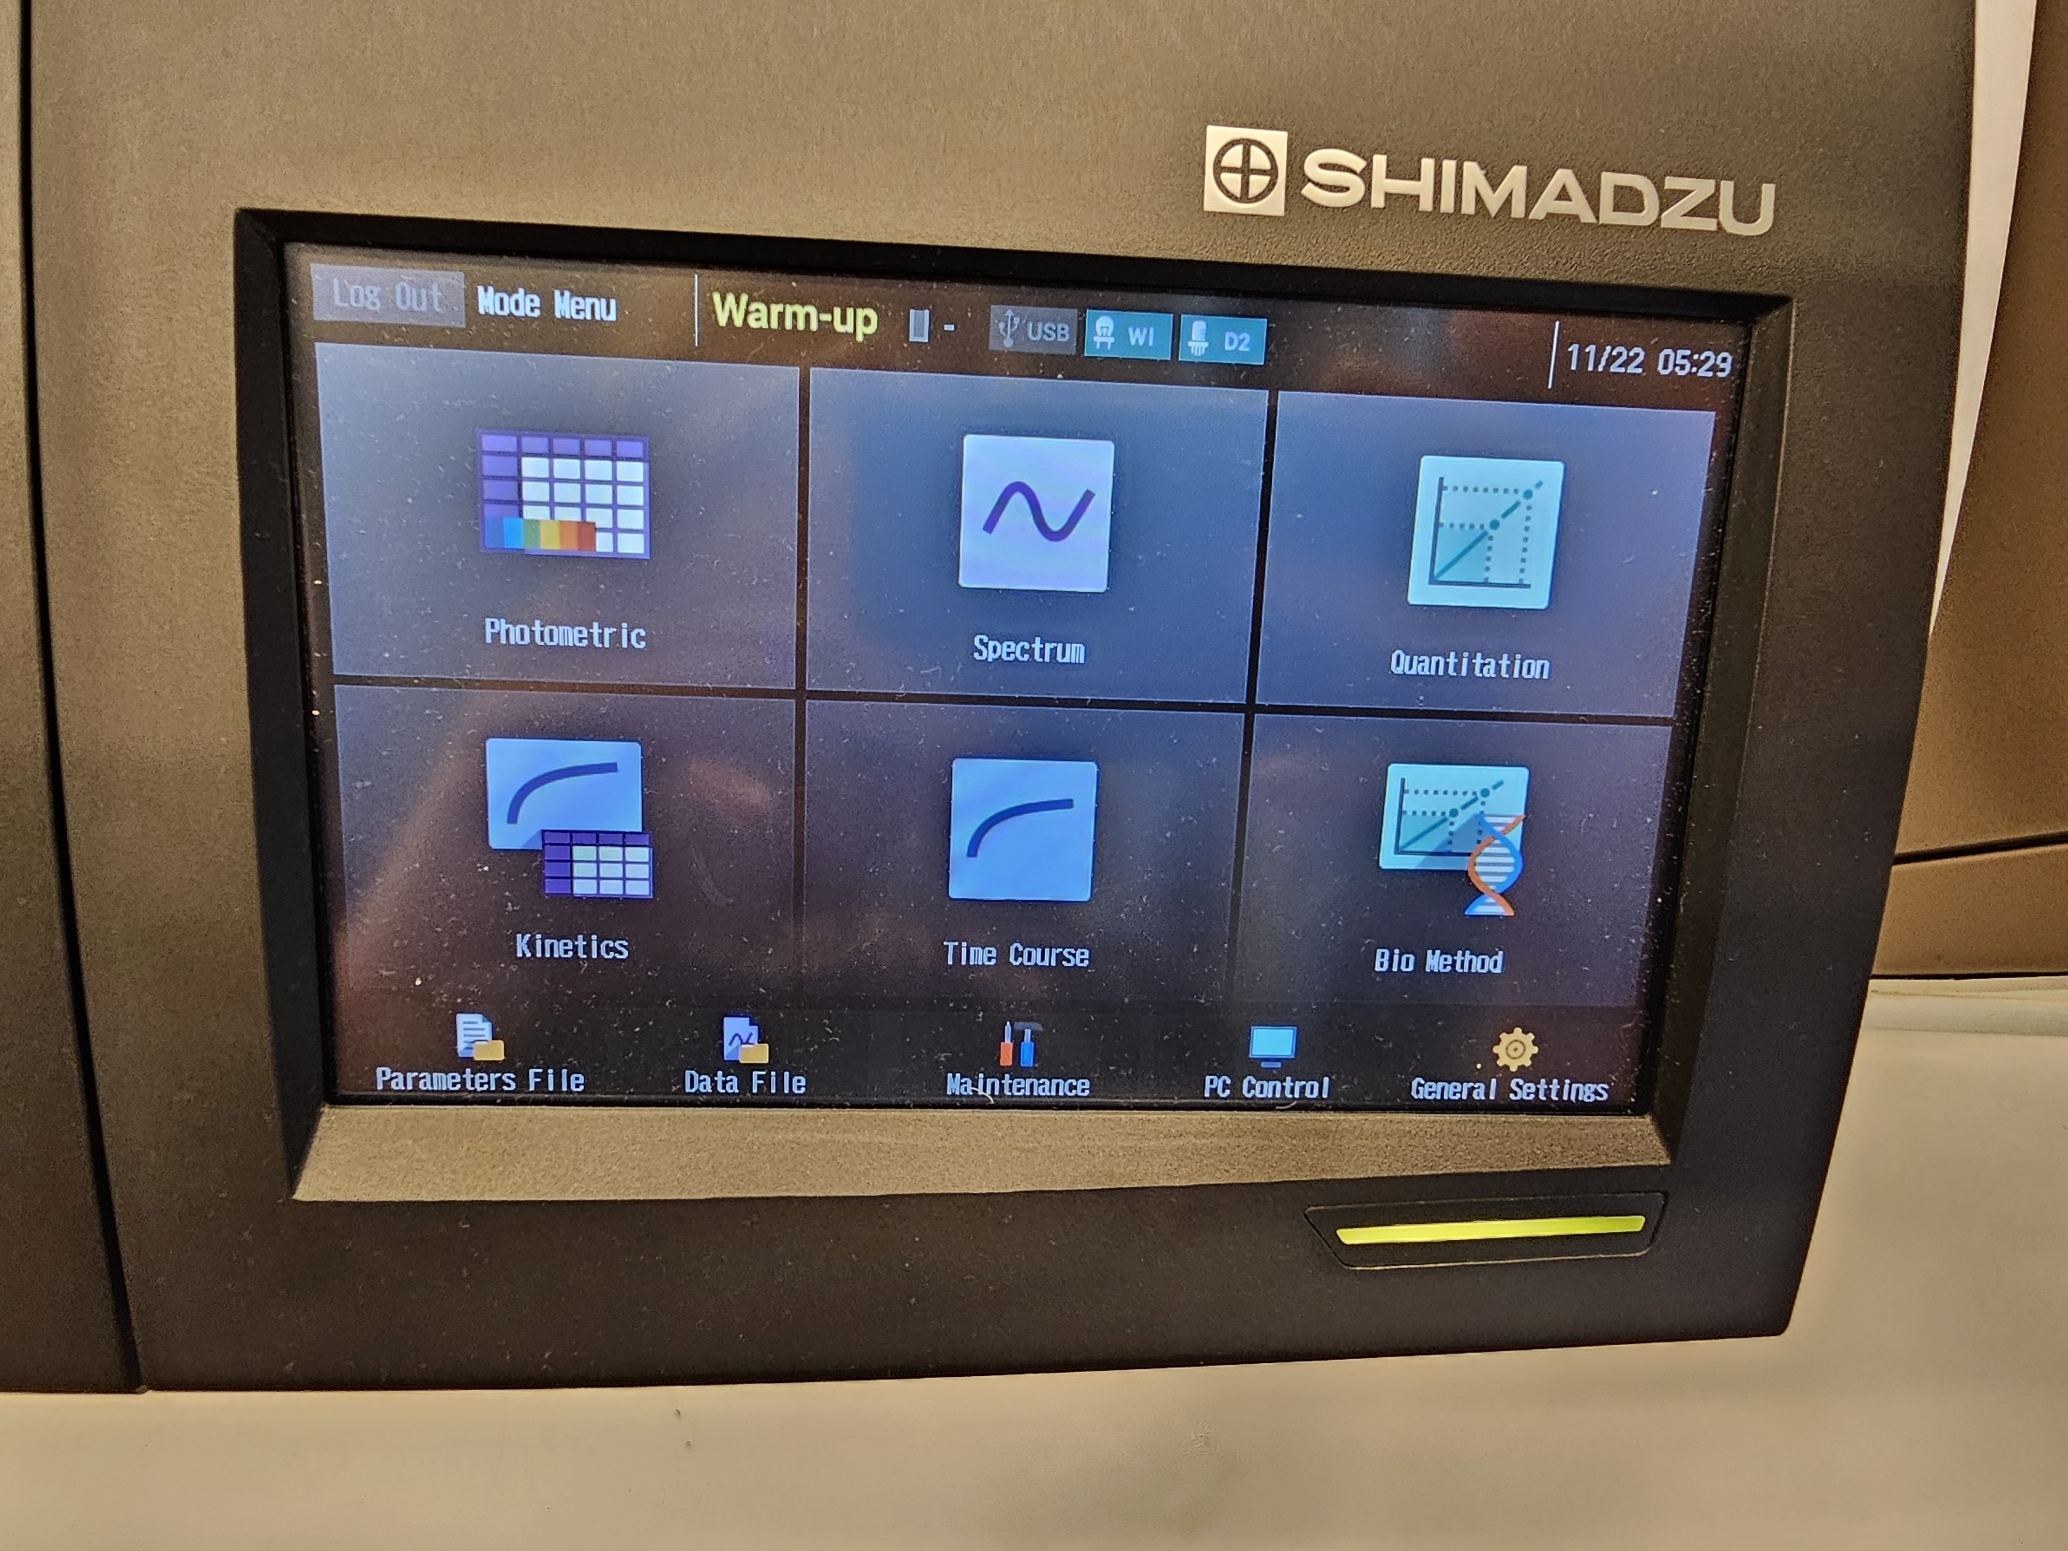
\includegraphics[width=\textwidth]{shimadzu_heating.jpg}
        \caption{Shimadzu UV-1900 warming up indicator}
        \label{fig:shimadzu_heating}
    \end{subfigure}
    \hfill
    \begin{subfigure}[b]{0.48\textwidth}
       \centering 
       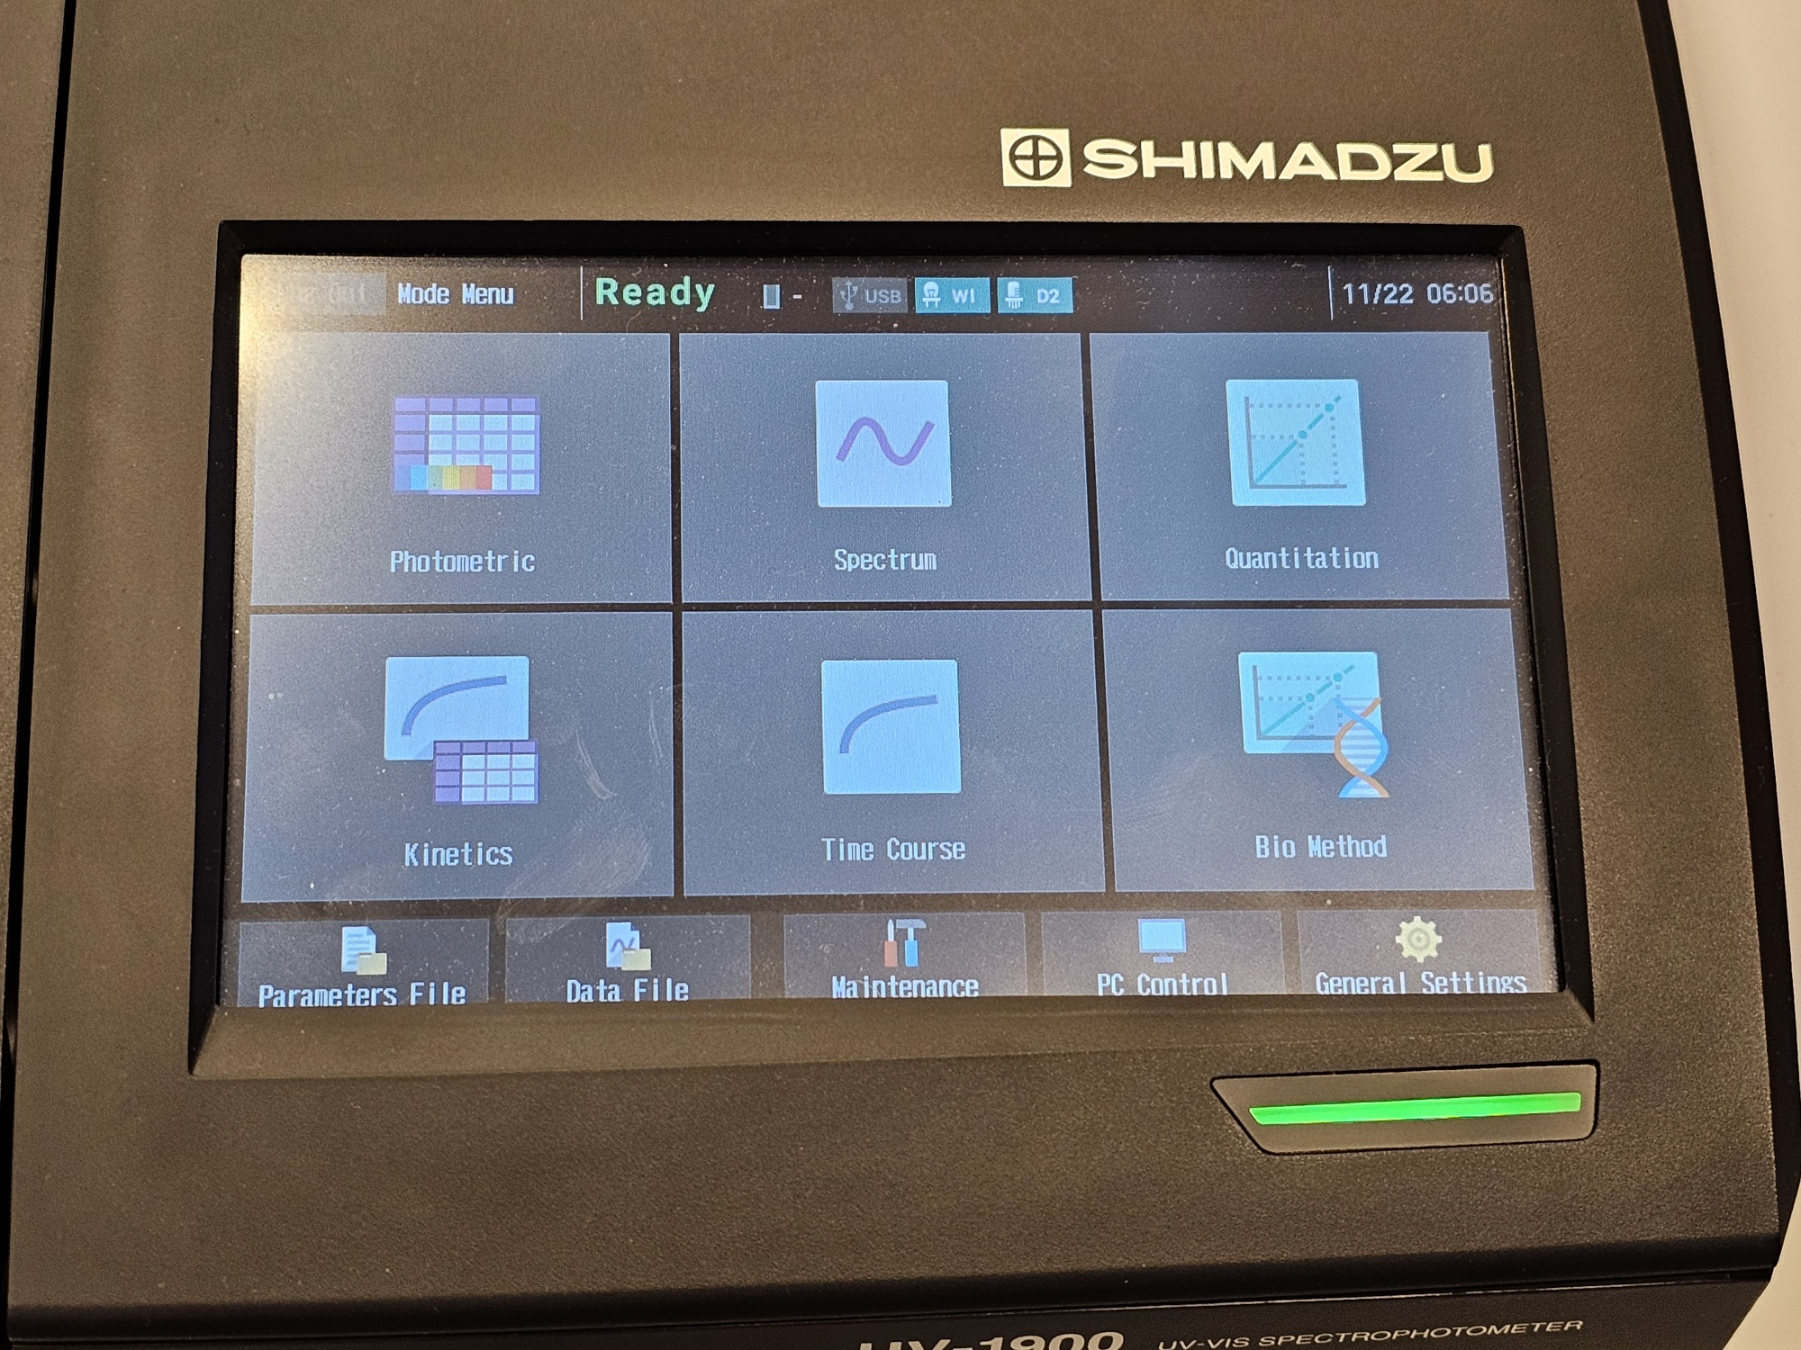
\includegraphics[width=\textwidth]{shimadzu_ready.jpg}
       \caption{Shimadzu UV-1900 ready and done warming up}
       \label{fig:shimadzu_ready}
    \end{subfigure}
    \caption{Shimadzu UV-1900 status indicator}
    \label{fig:shimadzu_status}
\end{figure}

After the instrument has heated up, a water reference measurement is then completed in the SpectroWorks\texttrademark\ software by Copenhagen Nanosystems (cphnano), with 2-3ml of DI water in the Nanocuvette\textsuperscript{TM} One.
The steps after this is then to prepare the measurements of vinyl chloride and DI water.

\begin{enumerate}
    \item 10 ml of DI water is added to a glass vial
    \item Added the corresponding volume of vinyl chloride to get the desired concentration. (e.g. 25 $\mu l$ to get a concentration of $ 4 \mu l / ml $)
    \item Then gently shaking the vinyl chloride and DI water solution for approximately 60 seconds.
    \item Takeing the enzyme Cytochrome P450 out of the freezer and start a stopwatch, to prevent the enzyme from being out of the freezer for more than 15 minutes.
    \item Weighed ~1.5-2mg of the enzyme.
    \item Then added a proportional amount of DI water to enzyme, meaning 1.5 mg of enzyme would require 1.5 ml of DI water.
    \item The enzyme and DI solution was then stirred gently for ~30 seconds, until there were no visible flakes of enzyme in the solution.
    \item Using a molar concentration of vinyl chloride to enzyme of $1.29 \times 10^5$, which is derived from the procedure sheet shown in the appendix \ref{appendix:protocol_vc}. The concentration was multiplied by a factor of 1-10$\times$, depending on the results of the previous experiment.
    \item When the enzyme had been added to the vinyl chloride solution, a stopwatch was started.
    \item The solution was gently shaken for approximately 30 seconds.
    \item 3 ml of this solution was then pipetted into a Nanocuvette\texttrademark\ One.
    \item The Nanocuvette\texttrademark\ One was then transferred into the spectrophotometer, starting with the A-side measurement, without the photonic crystal, in figure \ref{fig:nanocuvette_sides} an illustration shows the Nanocuvette\textsuperscript{TM} and the two sides of it.\label{step:measurement_start}

    \begin{figure}[H]
        \centering
        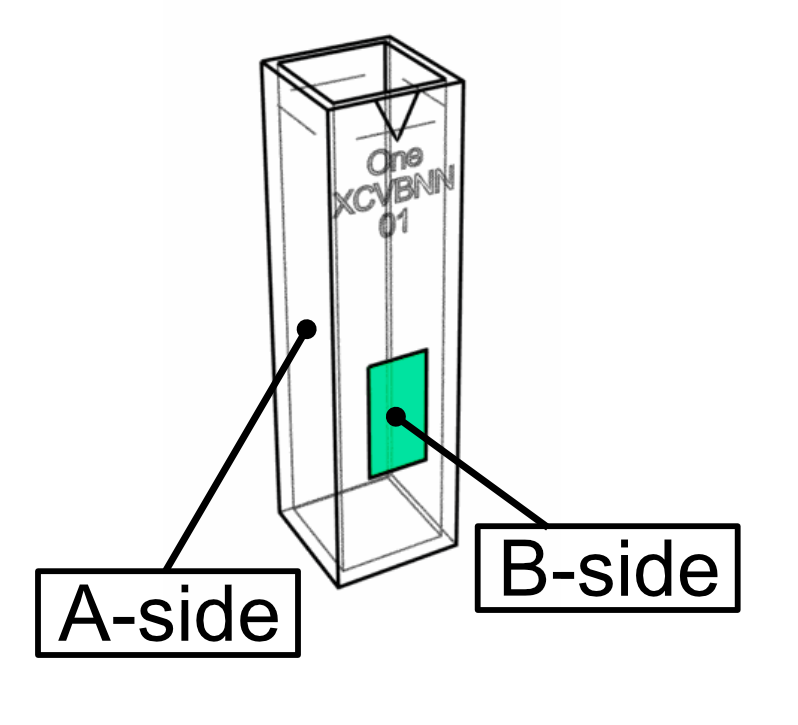
\includegraphics[width=0.5\linewidth]{nanocuvette_one_sides.png}
        \caption{A Nanocuvette\texttrademark\ One from cphnano\cite{cphnano_nanocuvette}}
        \label{fig:nanocuvette_sides}
    \end{figure}

    \item In the SpectroWorks\texttrademark\ software the water reference measurement done with DI water earlier, is selected.
    \item The A-side measurement was then carried out, according to the steps provided by the SpectroWorks\texttrademark\ software.
    \item The Nanocuvette\texttrademark\ One was then turned around to the B-side and the measurement was carried out again.
    \item The details for the measurement was then entered into SpectroWorks\texttrademark\:\label{step:measurement_end}
    \begin{itemize}
        \item Measurement number
        \item Current time (in minutes)
        \item DI volume
        \item Vinyl chloride volume
        \item Enzyme mass
    \end {itemize}
    \item The steps \ref{step:measurement_start} to \ref{step:measurement_end} was then carried with an approximate time gab of 1-2 minutes, until 60 minutes had passed.
\end{enumerate}

\subsubsection{Measuring with Water Care Guard suitcase}

\begin{figure}[H]
    \centering
    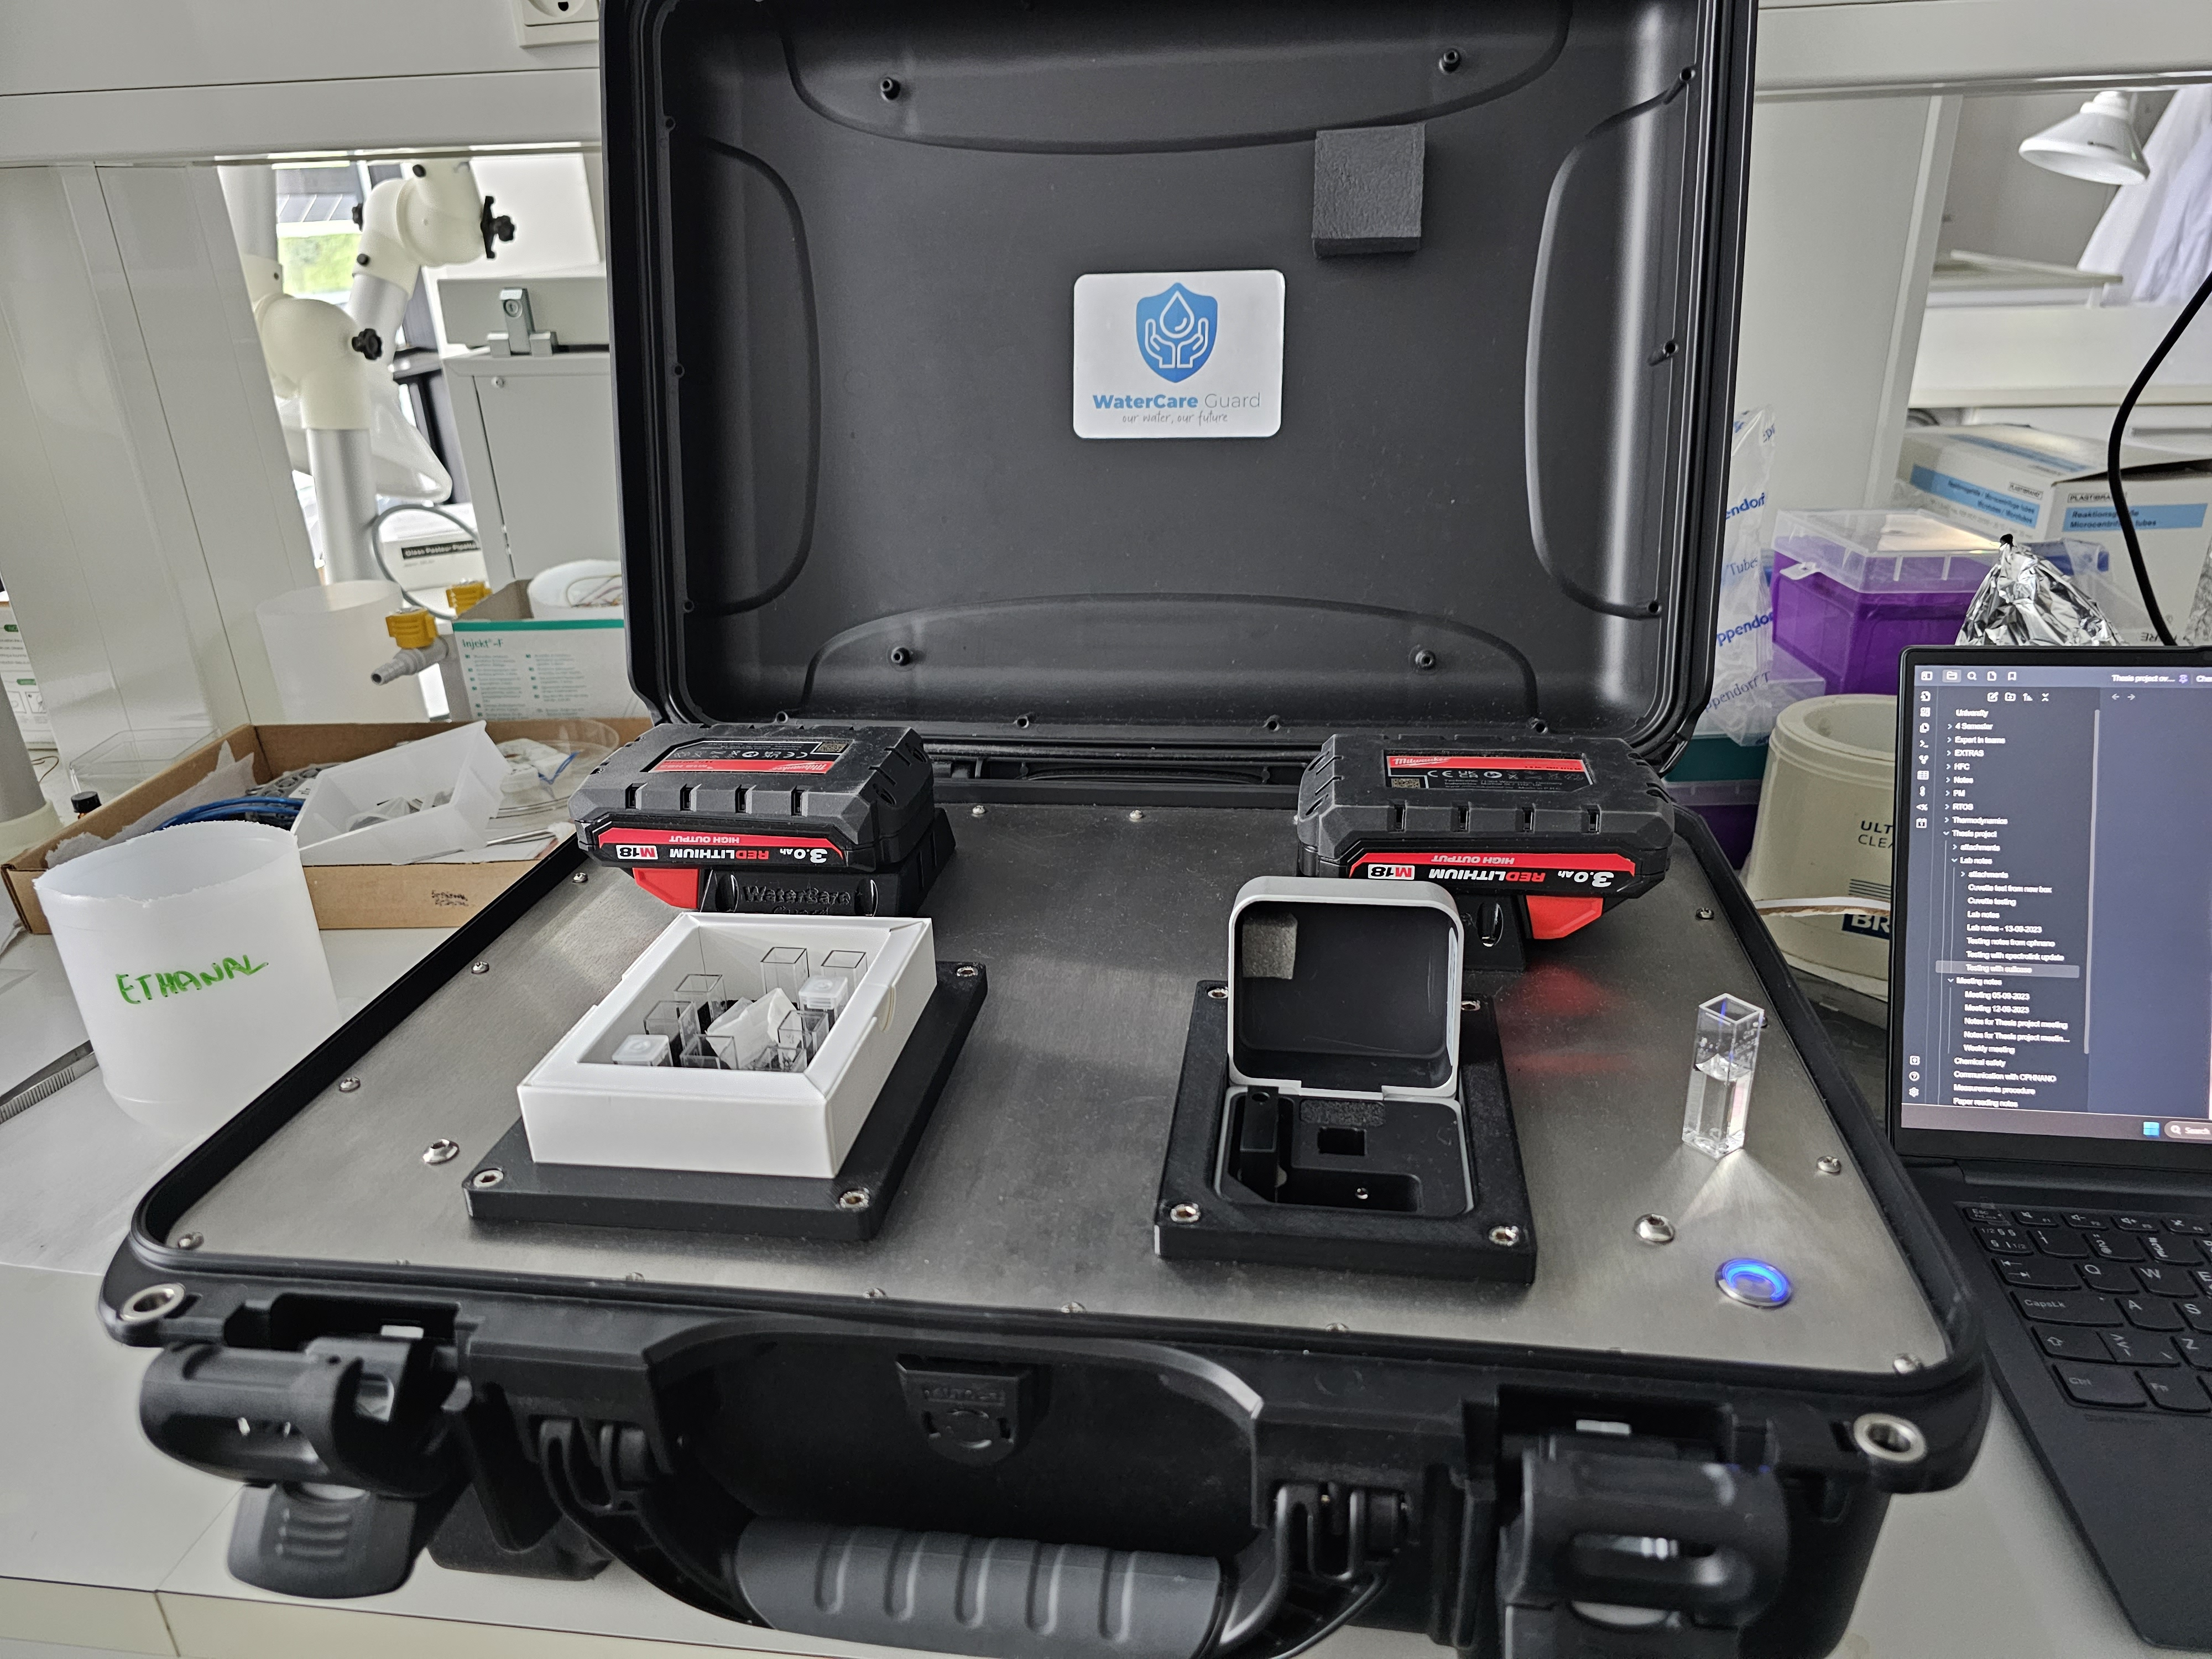
\includegraphics[width=0.8\textwidth]{wcg_suitcase.jpg}
    \caption{The Water Care Guard suitcase in the chemistry lab at SDU}
    \label{fig:wcg_suitcase}
\end{figure}

\subsubsection{Measuring with Shimadzu UV-1900}

\begin{figure}[H]
    \centering
    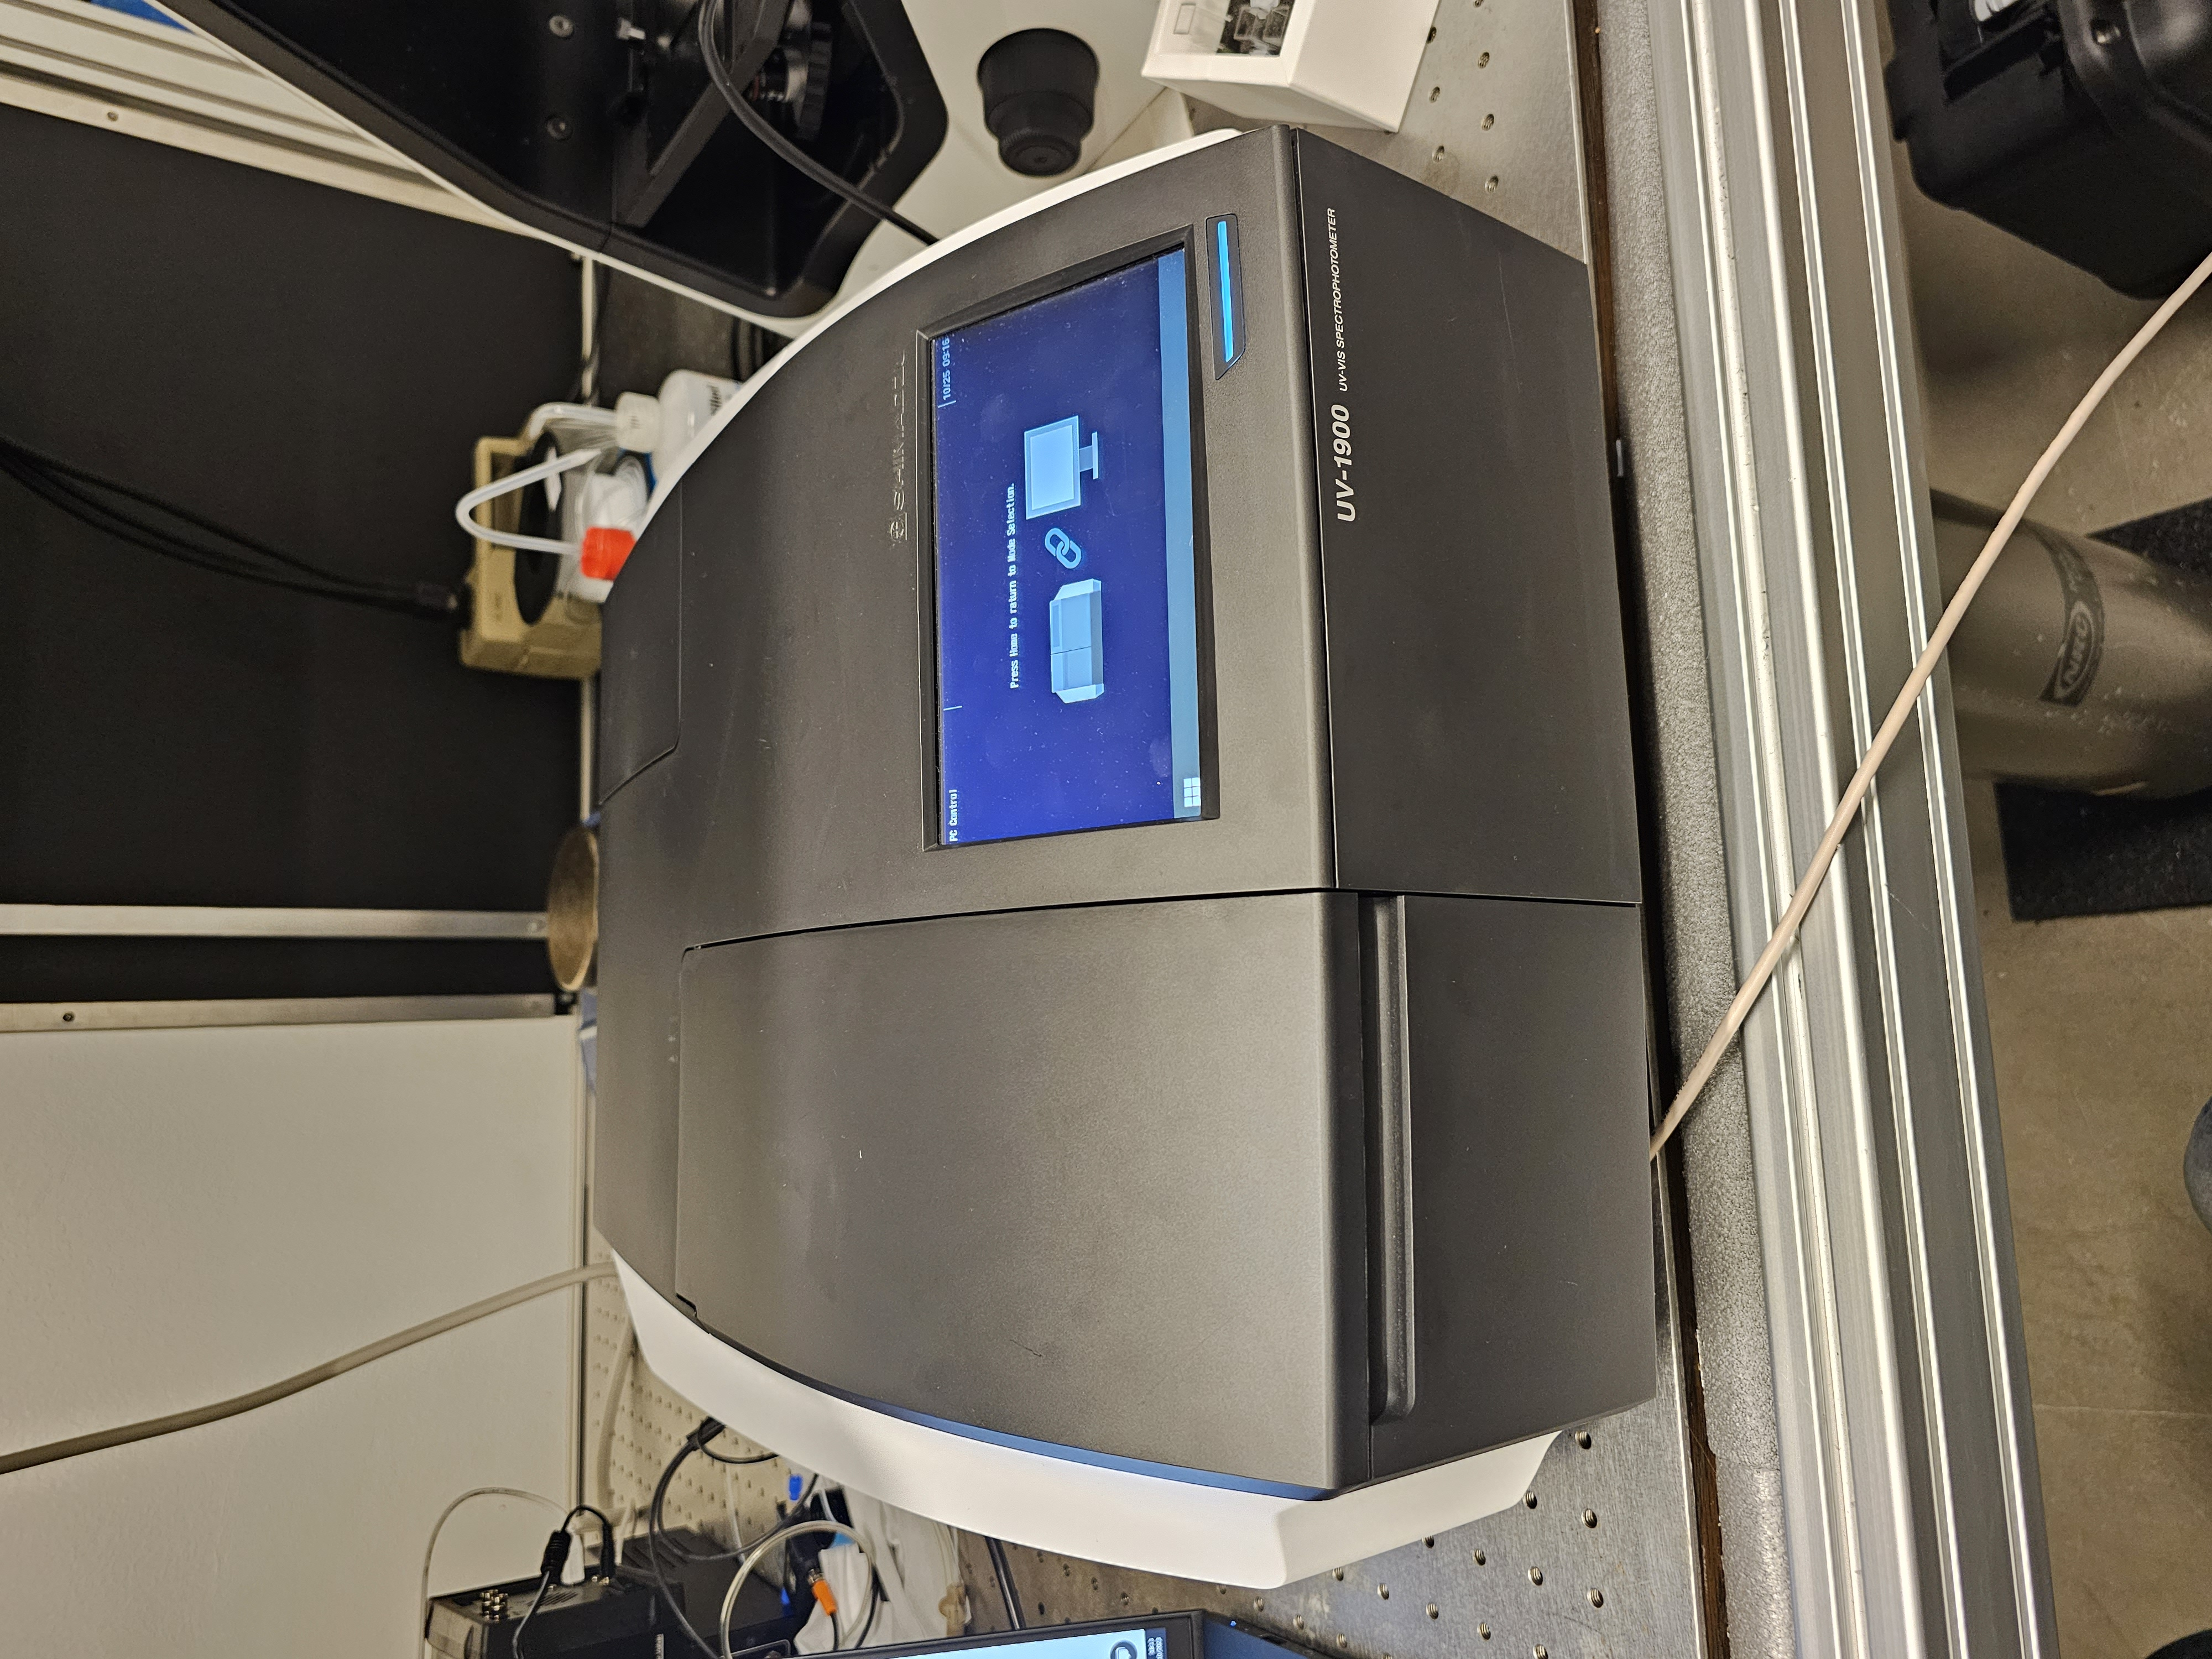
\includegraphics[width=0.8\textwidth, angle=270]{shimadzu_uv1900.jpg}
    \caption{Shimadzu UV-1900 spectrophotometer in the photonics lab at SDU}
    \label{fig:shimadzuuv1900}
\end{figure}

\subsection{Data analysis}
\subsection{Problems}

\newpage
\section{User interface}
The goal for the user interface was to have a simple solution for the user to be able to get the results of their measurements, without needing to understand the full program of SpectroWorks\texttrademark\ which is the backend for the handling the data, and taking the measurements.\\
SpectroWorks\texttrademark\ by cphnano is made to be able to handle a variety of measurement types and goals, like standard UV-Vis measurements, protein and enzyme concentrations, refractive index, particle size distributions etc.\cite{spectroworks}.
This is why the idea behind the user interface was to make it a simplified interface with SpectroWorks\texttrademark\, that was just a simple button to start the measurement and a display of the results.

\subsection{API Interface}
The API interface is written based on the python library for the API interface for SpectroWorks\texttrademark\ written by cphnano\cite{spectroworks_github}, it is written to be tailored to the needs of this project in an attempt to improve the performance of the system.
A full flowchart explaining how the program works with both the graphical user interface and the API interface is shown in the appendix \ref{appendix:api_interface} and in figure \ref{fig:flowchart_api}.\\

The first thing that the API inteface does is to establish a connection with the SpectroWorks\texttrademark\ API, an API key has been made in the SpectroWorks\texttrademark\ software that is being used to ensure that we are allowed to access the data.
In SpectroWorks\texttrademark\ we are able to define what projects the specific API key has access to, although in the API interface written, we have the option of choosing what project we are focusing on.\\

When the connection parameters has been set we are going to get a list of the projects available using the the API key, we then filter those projects and use only the ones we are interested in.
The get\_project method of the Connection class shown in code sample \ref{code:get_project}, uses the connection parameters to send a request to the SpectroWorks\texttrademark\ API, requesting a list of all the projects, they are then filtered based on if they are a part of the requested projects, it then returns the a Project class.

\begin{code}
\begin{minted}{python}
def get_project(self, project_name: str = None) -> Project:
    # load projects
    ## If you haven't loaded the projects earlier
    if self.projects is None:
        # Get response
        res = requests.get(
            self.url + 'list_projects',      # Determine request
            params={'api_key': self.api_key} # Add API key
        )
        if res.status_code != 200: # Response is not OK (200)
            # Throw an error, saying the connection is not successful.
            raise ConnectionError(json.loads(res.text)['message'])
        projects = json.loads(res.text)['message']['items']
        # Loop through the projects and filter based on our parameters
        for i, project in enumerate(projects):
            if project['project_name'] == project_name:
                return Project(self, projects[i])
\end{minted}
\captionof{listing}{get\_project method in the Connection class, written in Python.}
\label{code:get_project}
\end{code}
\medskip
In the projects class we can then get the properties of the Project, as well as getting the items associated with the given project.
An item is every individual measurement stored in SpectroWorks\texttrademark.
An example of an item as it is stored in SpectroWorks\texttrademark\ is shown below in figure \ref{fig:spectroworks_item}, in the image you can see the inputted sample attributes on the left side and the results of the measurements on the right side.

\begin{figure}[H]
    \centering
    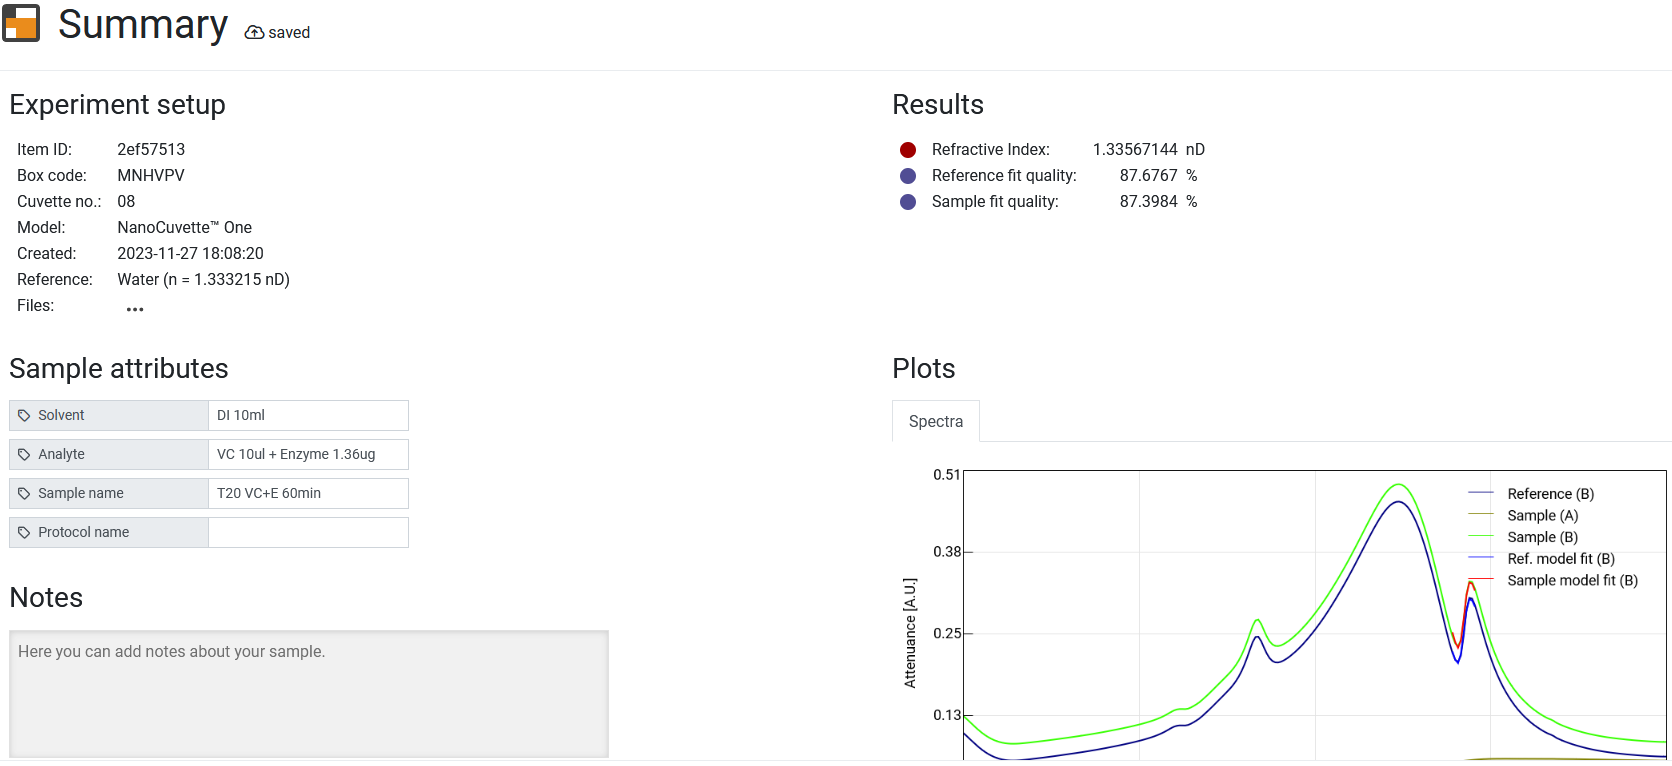
\includegraphics[width=\textwidth]{item_spectroworks.png}
    \caption{An item as shown in the SpectroWorks\texttrademark\ interface\cite{spectroworks_app}}
    \label{fig:spectroworks_item}
\end{figure}

Custom parameters for an item has been written into the sample parameters, like the volume of DI water, vinyl chloride, and the amount of enzyme in the solution, in addition the number for the measurement is written in with a T prefixed e.g. \textit{T20}, which indicates which measurements are from the same line of measurements, so that we can treat all the measurements with the same T number the same.
Lastly in the Sample name the time of the specific measurement is written as well, all these values can be extracted by the api interface program, the program uses a regular expression to extract the values.

\begin{code}
\begin{minted}{python}
## Test number
test_number = re.findall(r'T\d+', self.sample_name)
self.test_number = int(test_number[0][1:]) if test_number else None

## Measurement number
measurement_time = re.findall(r'\d+\.?\d*min', self.sample_name)
self.measurement_time = float(measurement_time[0][:-3]) if measurement_time else None
\end{minted}
\captionof{listing}{Example of getting the custom parameters using a regular expression from the sample attributes of the item.}
\label{code:custom_parameters}
\end{code}
\medskip

Using the \mintinline{python}{Project} class and \mintinline{python}{Item} class the program can get all the values it needs to be able to analyze the data.\\
The code for the SpectroWorks\texttrademark\ API interface and the website can be found on my github page (\url{https://github.com/Philip-Jorgensen/wcg_final_project})

\subsection{Graphical User Interface}
The graphical user interface is written as a locally hosted website, due to it being more accessible and easier to work with as the user.
As opposed to an application, a website can be accessed from any type of device assuming the device has access to the local network of the computer hosting the website.
This could mean how a tablet in the suitcase could be used as the interface for operating the Water Care Guard suitcase, an example for this is shown in figure \ref{fig:wcg_with_ipad} or the interface could be accessed from the users phone or computer.

\begin{figure}[H]
    \centering
    \includegraphics[width=0.9\textwidth]{wcg_suitcase_with_ipad.png}
    \caption{Illustration of the Water Care Guard suitcase with an iPad with the Graphical user interface.}
    \label{fig:wcg_with_ipad}
\end{figure}

\medskip

The website has been written with Python as the backend with the python framework Flask\footnote{\url{https://github.com/pallets/flask/}}, in addition the front end of the website is written in HTML and CSS.
The code for the graphical user interface can be found on my github (\url{https://github.com/Philip-Jorgensen/wcg_final_project/tree/main/gui/flask_based}).


\newpage
\section{Conclusion}

\newpage

\renewcommand*{\UrlFont}{\rmfamily}
\printbibliography[heading=bibintoc, title={Bibliography}]

\section{Appendix}
% Add the code here, and a flowchart version to describe the logic

\subsection{spectroworks\_api\_interface.py}\label{appendix:api_interface}
\begin{figure}[H]
    \centering
    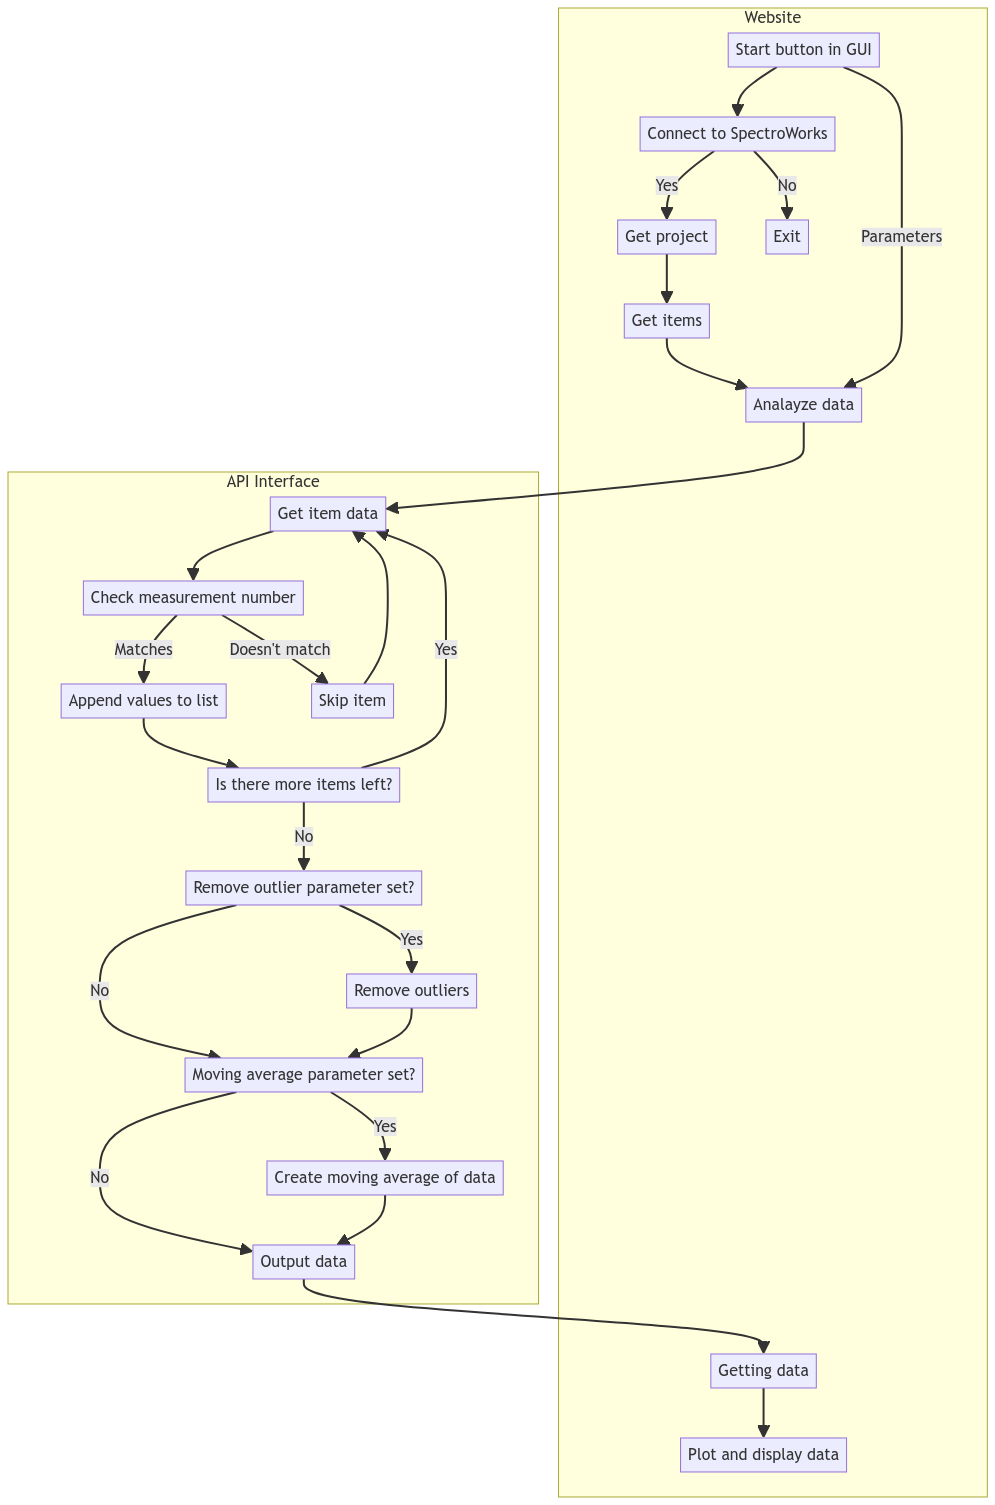
\includegraphics[width=\textwidth]{flowchart_api_white.png}
    \caption{The flowchart for the website and SpectroWorks\texttrademark\ api interface}
    \label{fig:flowchart_api}
\end{figure}

\subsection{Protocol how to prepare VC + Enzyme concentration in water based on molar ratio 1:6 and measure the RI}\label{appendix:protocol_vc}
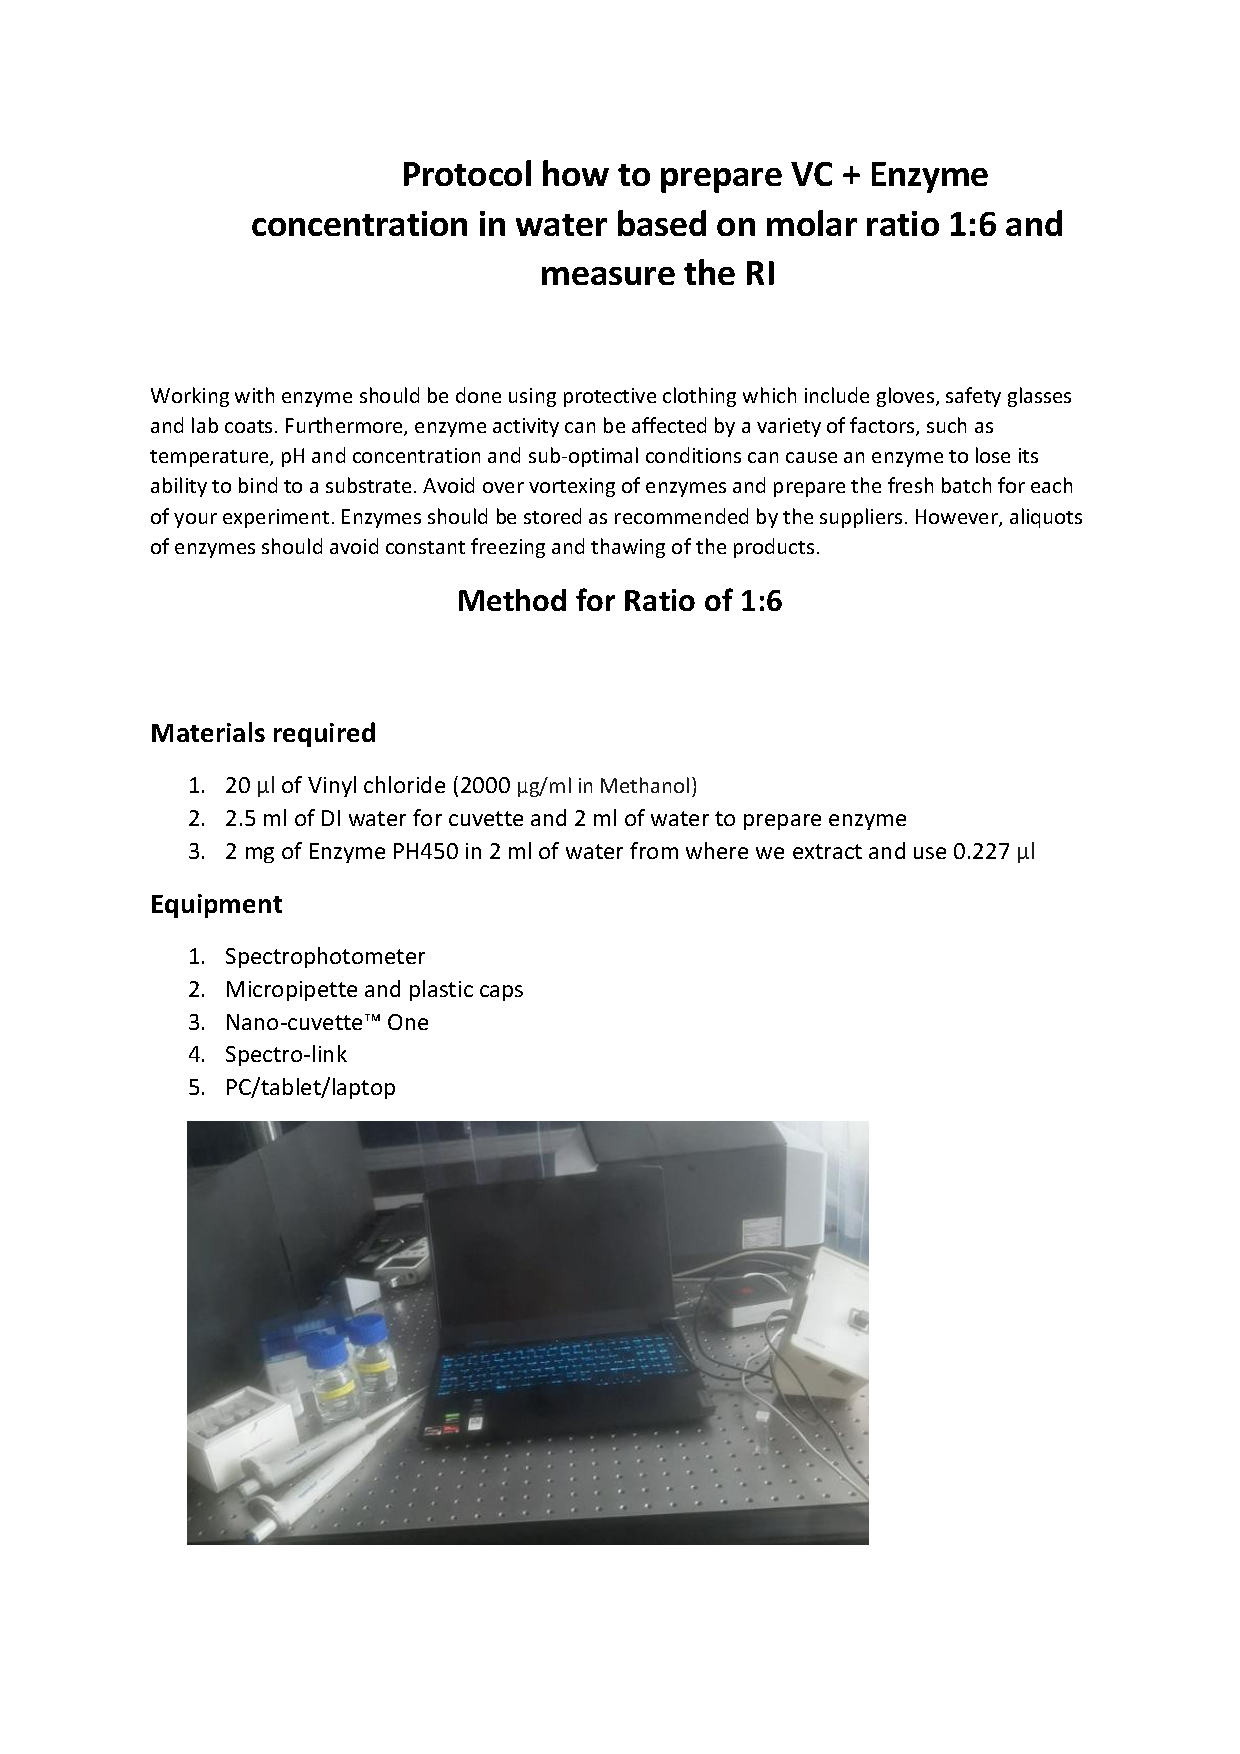
\includepdf[pages=-]{appendix/Protocol_for_working_enzyme_kinetics.pdf}

\end{document}